\subsection{Light GCN based Aspect-level Collaborative Filtering}
LGC-ACF (Light GCN based Aspect-level Collaborative Filtering) is a recommendation model developed by Denghua Mei et. al that utilizes LightGCN and side information \cite{LGC-ACF}.
As described in \autoref{sec:pre-specialization-paper} in our pre-specialization paper tried to extend LightGCN by changing the input parameters to include a more diverse graph that included side information.
These results showed that inputting a more diverse graph was not feasible to improve the results of LightGCN \cite{Pre-specialisation}.
LGC-ACF utilizes side information differently, where they include multiple aspect-level user-item interaction graphs and showed improvements of LightGCN between 2\% and 14\% in their experiments \cite{LGC-ACF}.
On \autoref{fig:lgc-acf} the model of LGC-ACF can be seen.
The input to the model is a user-movie graph and a user-director graph, where the users are the same.
In the user-movie graph, 1 is inserted if there is a connection between a user and a movie.
For the user-director graph, the number of interactions between the user and director is inserted.
An example of the director embedding can be seen on \autoref{eq:director-embedding}, where $D$ denotes the aspect of director, $N$ denotes the number of users, and $M_D$ denotes the number of directors.
\begin{equation}
    E^D = [e_{u_1}^D, ... , e_{u_n}^D, e_{i_1}^D, ..., e_{i_{M_D}}^D]
    \label{eq:director-embedding}
\end{equation}
It is possible to input an arbitrary number of input graphs, as long as the users are the same.
The box with LightGCN embedding and Layer combination is essentially what happens on \autoref{fig:gcn-figure} except for the final prediction.
When the embeddings have been created for the user-movie graph and user-director graph, a weighted summation is done.
The weighted summation can be seen on \autoref{eq:LGC-ACF-sum}, where G is the total amount of input graphs and $\alpha_k$ is set to $1/K + 1$.
This is identical to the layer combination method presented by LightGCN \cite{lightgcn}.
\begin{equation}
    \mathbf{e}_u = \sum_{g=0}^{G} \alpha_k \mathbf{e}_u^{(g)},
    \label{eq:LGC-ACF-sum}
\end{equation}
\begin{figure*}[h!]
    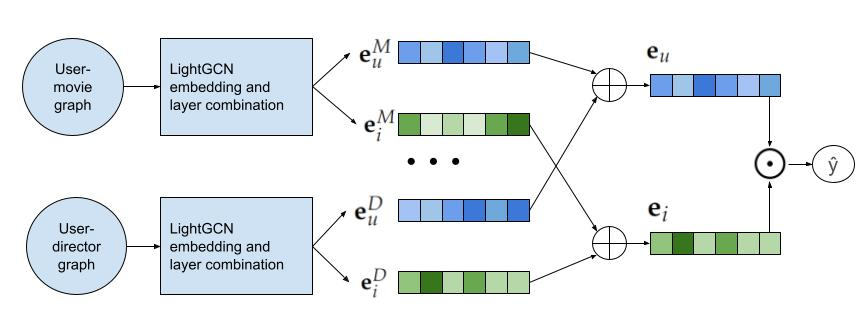
\includegraphics[width=1.1\textwidth]{figures/LGC-ACF.jpg}
    \centering
    \caption{LGC-ACF where $\odot$ is the dot product, and $\oplus$ is the weighted summation.}
    \label{fig:lgc-acf}
\end{figure*}
